\documentclass{beamer}
%https://www.overleaf.com/project/5e98d848e782e700010bb104
% Choose how your presentation looks.
%
% For more themes, color themes and font themes, see:
% http://deic.uab.es/~iblanes/beamer_gallery/index_by_theme.html
%
\mode<presentation>
{
  \usetheme{default}      % or try Darmstadt, Madrid, Warsaw, ...
  \usecolortheme{default} % or try albatross, beaver, crane, ...
  \usefonttheme{default}  % or try serif, structurebold, ...
  \setbeamertemplate{navigation symbols}{}
  \setbeamertemplate{caption}[numbered]
} 

\usepackage[english]{babel}
\usepackage[utf8x]{inputenc}
\usepackage{mathtools}
\usepackage{color}
\usepackage{amsmath}

\newcommand{\qbin}[2]{\begin{bmatrix}{#1}\\ {#2}\end{bmatrix}_q}

\title{Applications of Numerical PDEs in Image Processing and Computer Vision}
\author{Lindsey Grigsby}
\institute{University of Florida}
\date{Spring 2020}

\begin{document}

\begin{frame}
  \titlepage
\end{frame}


\section{Introduction}

%%%%%%%%%%%%%%%%%%%%%%%%%%%%%%%%
\begin{frame}{Introduction}

    \begin{block}{Image processing}
    \begin{itemize}
        \item the transformation of an input image into an output image
        \item e.g. compression, rotation, blurring, edge detection
    \end{itemize}
    \end{block}
    
    \begin{block}{Computer vision}
    \begin{itemize}
      \item uses image processing algorithms to complete tasks related to understanding an image
      \item e.g. edge detection, motion tracking, object recognition
    \end{itemize}
    \end{block}
    
    several good libraries, e.g. OpenCV (C++/Python)

\end{frame}

%%%%%%%%%%%%%%%%%%%%%%%%%%%%%%%%
\begin{frame}{Mathematical operations on images}
    
    \begin{itemize}
        \item Can consider an image:
        \begin{itemize}
            \item a \textit{length}$\times$\textit{width} matrix of pixels
            \item or, an intensity function $I(x,y)$ describing the intensity at each pixel $(x,y)$
        \end{itemize}
        \item Operations
        \begin{itemize}
            \item easy to imagine how to convert to grayscale, rotate, etc
            \item easy to imagine what multiplication by a constant, taking the transpose, etc, will do
        \end{itemize}
        \item more interesting tasks can also be intuitive
        \item e.g. edge detection 
    \end{itemize}

\end{frame}

%%%%%%%%%%%%%%%%%%%%%%%%%%%%%%%%
\begin{frame}{A simple example involving partial derivatives}
    
    \begin{figure}[h!]
            \centering            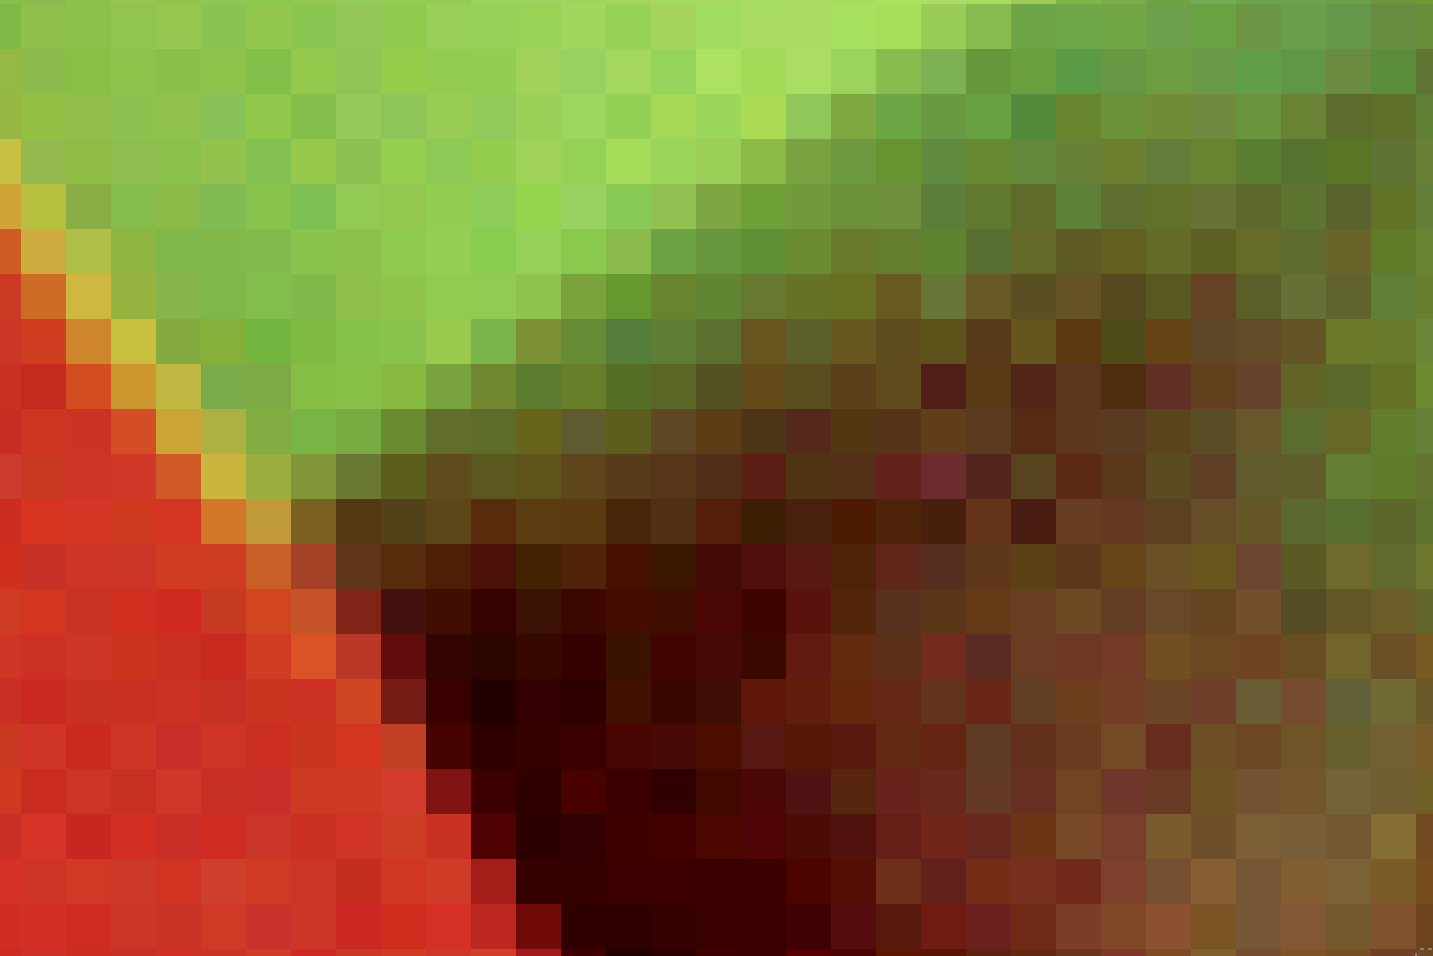
\includegraphics[scale=0.15]{edgedet2.png}
            \caption{What is an edge? Try: a curve such that along each line perpendicular to it, pixel values change very quickly. (Then there are 2 edges here.)}
    \end{figure}

\end{frame}

%%%%%%%%%%%%%%%%%%%%%%%%%%%%%%%%
\begin{frame}{A simple example involving partial derivatives}
    
    \begin{figure}[h!]
            \centering            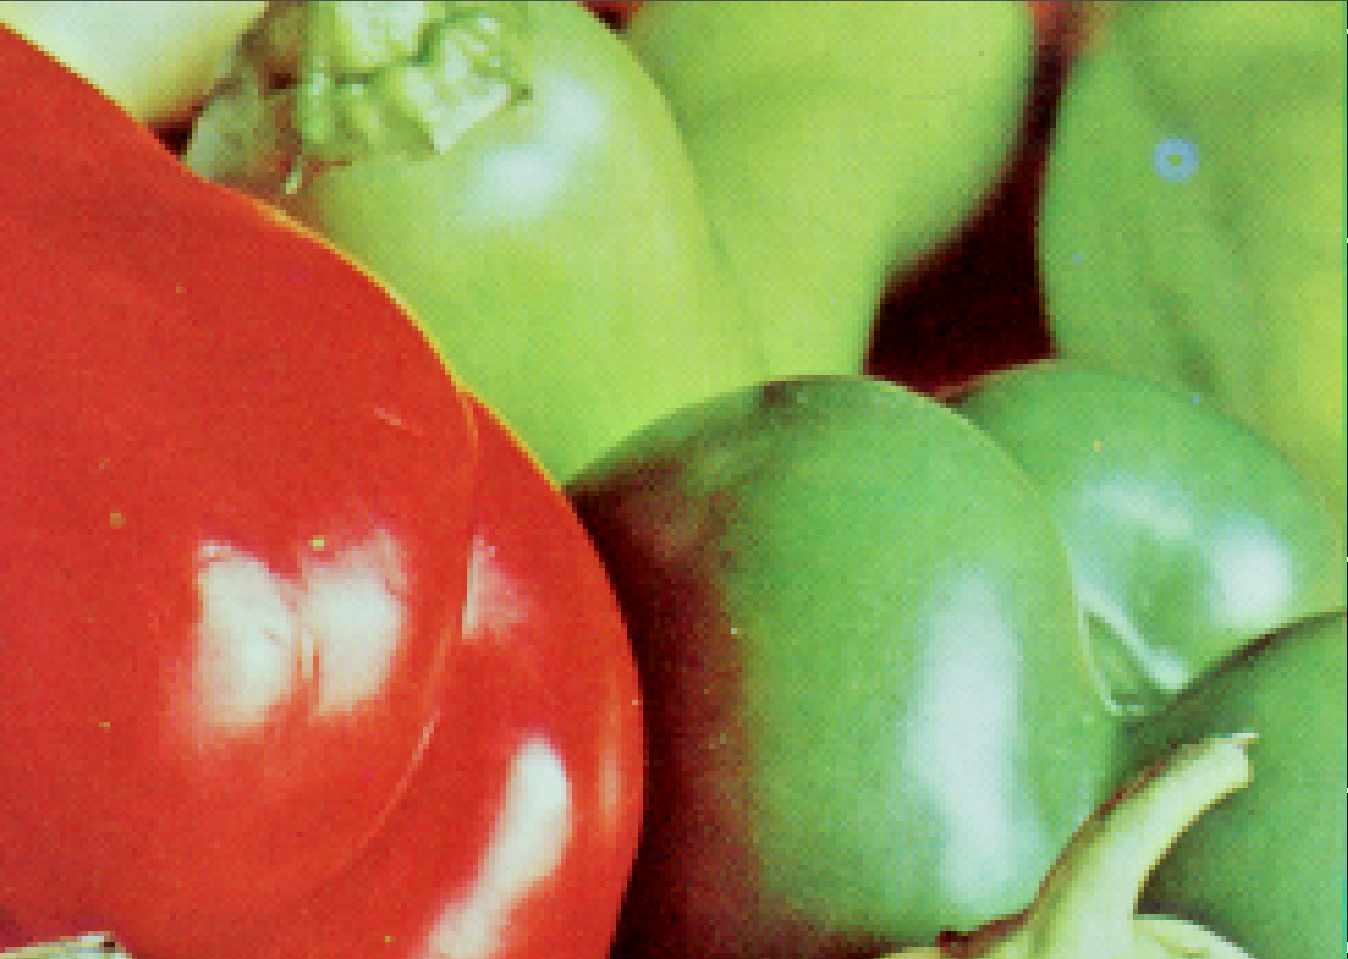
\includegraphics[scale=0.15]{edgedet1.png}
            \caption{Zooming out, the edges detected via this method make sense.}
    \end{figure}

\end{frame}

%%%%%%%%%%%%%%%%%%%%%%%%%%%%%%%%
\begin{frame}{A simple example involving partial derivatives}
    
    Formally: 
    \begin{itemize}
        \item consider the image in terms of its intensity function $I(x,y)$
        \item say $(x,y)$ is part of an edge if $||\nabla I(x,y)||$ is a local max (recall that $||\nabla I(x,y)||$ $\Longleftrightarrow$ rate of increase in the direction of fastest increase)
        \item this $+$ some simple refining steps is Canny edge detection
    \end{itemize}
    \begin{figure}[h!]
            \centering            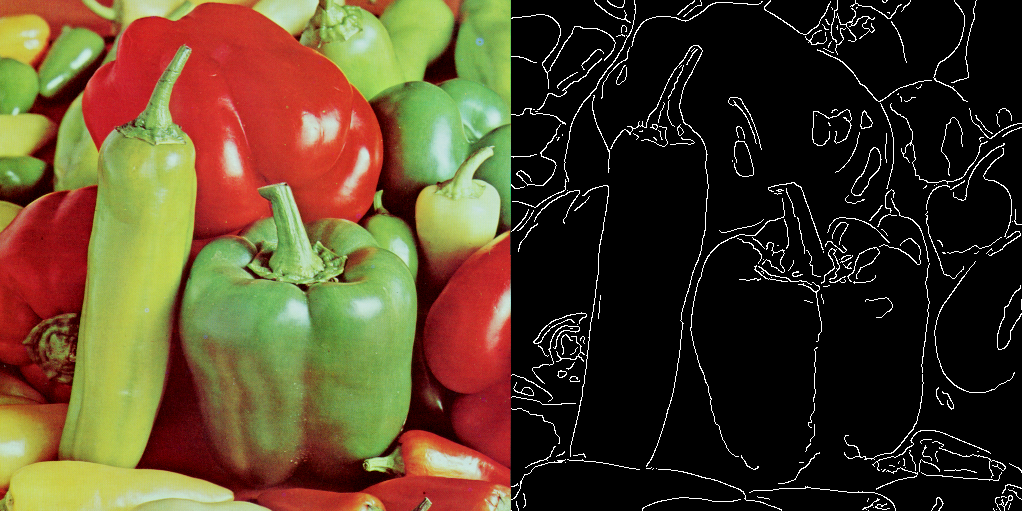
\includegraphics[scale=0.25]{edgedetect1.png}
            \caption{The result of Canny edge detection}
    \end{figure}

\end{frame}

\section{Examples of PDEs in image processing and computer vision}

\begin{frame}
  \vfill
  \centering
  \begin{beamercolorbox}[sep=8pt,center,shadow=true,rounded=true]{title}
    \usebeamerfont{title}{Examples of PDEs in image processing and computer vision}\par%
  \end{beamercolorbox}
  \vfill
\end{frame}

%%%%%%%%%%%%%%%%%%%%%%%%%%%%%%%%
\begin{frame}{Image segmentation}
    
    \begin{itemize}
        \item separates an image into regions based on some criteria (e.g. distinct objects)
        \item many methods, including several efficient PDE methods
    \end{itemize}
    
    \begin{figure}[h!]
        \centering            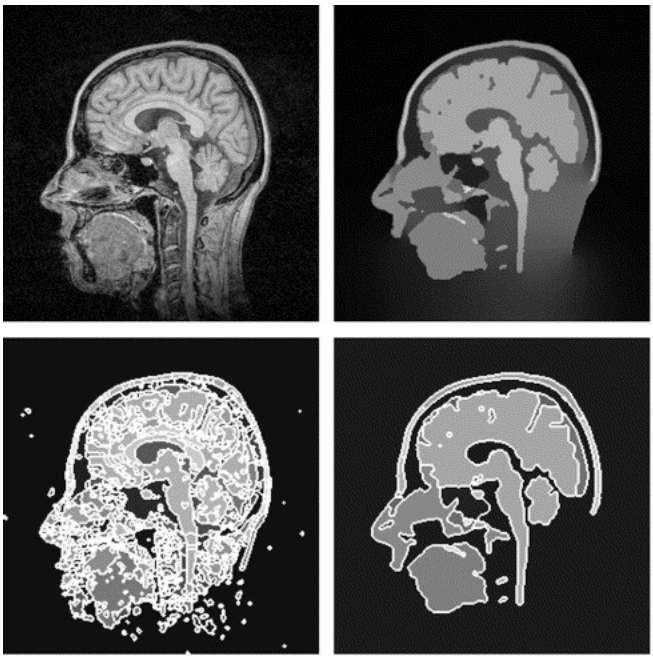
\includegraphics[scale=0.22]{segmentation2.png}
        \caption{``Efficient image segmentation using partial differential equations and morphology'', Weickert}
    \end{figure}

\end{frame}

%%%%%%%%%%%%%%%%%%%%%%%%%%%%%%%%
\begin{frame}{Inpainting}
    
    \begin{itemize}
        \item removes large imperfections from images
        \item two main PDE-related algorithms - one based on Navier-Stokes, and another based on the ``fast marching method''
    \end{itemize}
    
    \begin{figure}[h!]
        \centering            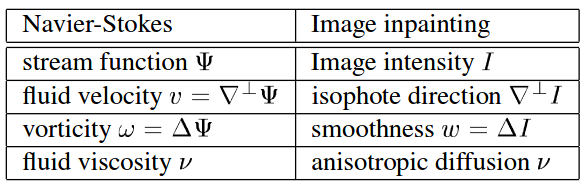
\includegraphics[scale=0.35]{inpainting4.png} \caption{``Navier-Stokes, fluid dynamics, and image and video inpainting'', Bertalmio.}
    \end{figure}

\end{frame}

%%%%%%%%%%%%%%%%%%%%%%%%%%%%%%%%
\begin{frame}{Inpainting}
    
    \begin{figure}[h!]
        \centering            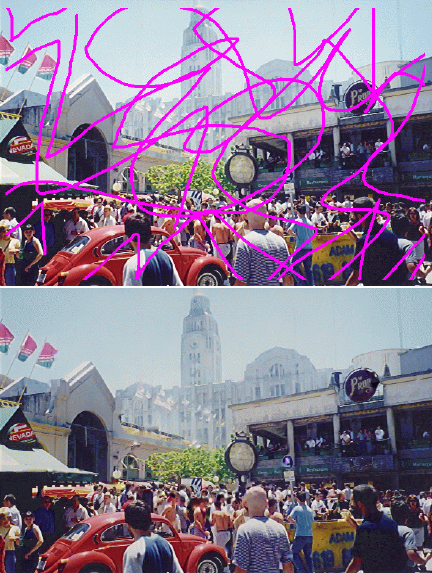
\includegraphics[scale=0.35]{inpainting1.png}
        \caption{An example from the same paper}
    \end{figure}

\end{frame}

%%%%%%%%%%%%%%%%%%%%%%%%%%%%%%%%
\begin{frame}{Anisotropic diffusion}
    
    \begin{itemize}
        \item removes noise from an image without blurring details necessary for interpreting the image (like edges)
        \item related to the heat equation
    \end{itemize}
    
    \begin{figure}[h!]
            \centering            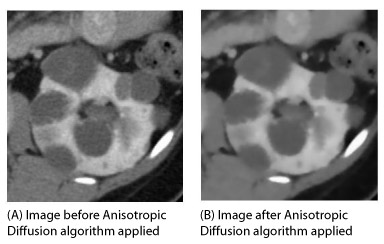
\includegraphics[scale=0.6]{anisodif1.jpg}
            \caption{Noise is reduced without blurring edges}
    \end{figure}

\end{frame}

\section{Anisotropic Diffusion}

\begin{frame}
  \vfill
  \centering
  \begin{beamercolorbox}[sep=8pt,center,shadow=true,rounded=true]{title}
    \usebeamerfont{title}{Anisotropic Diffusion}\par%
  \end{beamercolorbox}
  \vfill
\end{frame}

%%%%%%%%%%%%%%%%%%%%%%%%%%%%%%%%
\begin{frame}{Motivation}
    
    
    \begin{itemize}
        \item one way to reduce noise is via Gaussian diffusion (blurring)
        \item but, this blurs everything evenly
    \end{itemize}
    
    \begin{figure}[h!]
            \centering            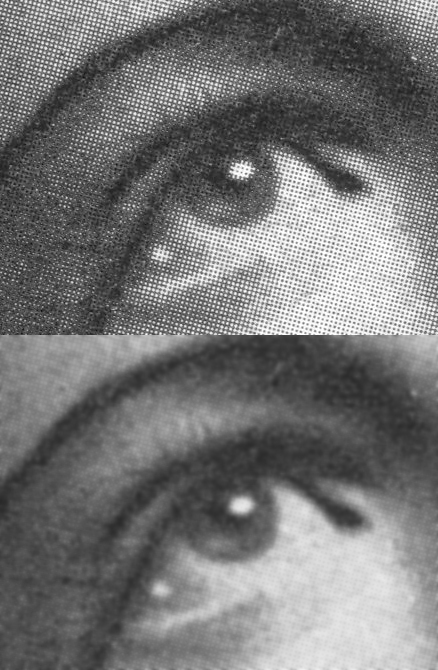
\includegraphics[scale=0.9]{gaussianblur.jpg}
            \caption{Original image smoothed using Gaussian diffusion}
    \end{figure}

\end{frame}

%%%%%%%%%%%%%%%%%%%%%%%%%%%%%%%%
\begin{frame}{Motivation}
    
    The fix: consider what Gaussian diffusion is in terms of PDEs. 
    \begin{itemize}
        \item clear analogy with heat transfer: 
            \begin{align*}
                \text{heat equation}&\Longleftrightarrow\text{gaussian diffusion equation}\\
                \frac{\delta u}{\delta t} = \alpha\Delta u &\Longleftrightarrow \frac{\delta I}{\delta t} = c\Delta I
            \end{align*}
        where
            \begin{align*}
                u(x,y,t)\,\,\,\small\text{(temp at time t)}&\Longleftrightarrow I(x,y,t)\,\,\,\small\text{(pixel value at time t)}
            \end{align*}
        and 
            \begin{align*}
                \alpha\,\,\,\small\text{(diffusivity of the medium)}&\Longleftrightarrow c\,\,\,\small\text{(diffusion coefficient)}
            \end{align*}
    \end{itemize}
    
\end{frame}

%%%%%%%%%%%%%%%%%%%%%%%%%%%%%%%%
\begin{frame}{Motivation}
    
    In the Gaussian diffusion equation
    \begin{equation*}
        \frac{\delta I}{\delta t} = c\Delta I= div\left(c\nabla I\right)
    \end{equation*}
    (note: $\Delta=$ Laplacian and $\nabla=$ gradient),
    
    \begin{itemize}
        \item $c$ controls how much the image blurs
        \item so if we want to prevent blurring in particular places (like edges), we could try making $c$ a function
    \end{itemize}
    
\end{frame}

%%%%%%%%%%%%%%%%%%%%%%%%%%%%%%%%
\begin{frame}{The anisotropic diffusion equation}
    
    Call this modified equation,
    \begin{align*}
        \frac{\delta I}{\delta t} &= div\left(c(x,y,t)\nabla I\right)\\
        &=\nabla c\cdot \nabla I+c(x,y,t)\Delta I,
    \end{align*}
    the anisotropic diffusion equation. We want it to uniquely define a family of images (parametrized by $t$) which can be easily computed.
    
    \begin{itemize}
        \item do there even exist (non-constant) $c$ so that this problem is well-posed and numerically stable?
        \item if so, will one of these $c$'s improve on Gaussian noise reduction?
    \end{itemize}
    
\end{frame}

%%%%%%%%%%%%%%%%%%%%%%%%%%%%%%%%
\begin{frame}{Specializing the problem}
    
    \begin{block}{}Perona and Malik investigated anisotropic diffusion in 1987.\end{block}
    
    \begin{block}{}They formalized what they wanted out of the family of images (i.e., what ``blur while preserving edges'' means)\end{block}
    
    \begin{block}{Example of a tree against sky}
        \begin{itemize}
            \item instead of ``edges'', talk about region boundaries at different resolutions
            \item want a family of images such that 
                \begin{itemize}
                    \item First, boundaries between details on individual leaves are blurred. Then boundaries between leaves are blurred. Then sky and tree are blurred together.
                \end{itemize}
        \end{itemize}
    \end{block}
    
\end{frame}

%%%%%%%%%%%%%%%%%%%%%%%%%%%%%%%%
\begin{frame}{Choosing the diffusion coefficient $c(x,y,t)$}
    
    \begin{block}{}
        If somehow we knew exactly where the region boundaries were at time any time $t$, then we could choose
            \begin{equation*}
                c(x,y,t)=\begin{cases}
                    1 & (x,y,t)\in\{\text{interior of some region}\}\\
                    0 & (x,y,t)\in\{\text{boundary of some region}\}.
                \end{cases}
            \end{equation*}
    \end{block}
    
    \begin{block}{}
        \begin{itemize}
            \item Then at each time $t$, the interiors of regions would blur and the boundaries would not - exactly what we want.
            \item But, we don't generally have this region info. 
        \end{itemize}
    \end{block}

\end{frame}

%%%%%%%%%%%%%%%%%%%%%%%%%%%%%%%%
\begin{frame}{Choosing the diffusion coefficient $c(x,y,t)$}
    
    \begin{block}{}
        If somehow we could estimate where the region boundaries were at any time $t$, then we could choose  $c(x,y,t)$ to be a decreasing function (with values between $0$ and $1$) of how likely it is that $(x,y,t)$ is part of a boundary.
    \end{block}
    
    \begin{block}{}
        \begin{itemize}
            \item Then at each time $t$, the probably-interiors of regions would blur significantly and the probably-boundaries would blur less.
            \item Can we get these  boundary estimations? 
        \end{itemize}
    \end{block}

\end{frame}

%%%%%%%%%%%%%%%%%%%%%%%%%%%%%%%%
\begin{frame}{Choosing the diffusion coefficient $c(x,y,t)$}

    \begin{block}{}
        We already have one way to estimate boundaries, using the fact that $||\nabla||=$ rate of increase in the direction of fastest increase.
    \end{block}
    
    \begin{block}{}
        So we can choose
        \begin{equation*}
            c(x,y,t)=g(||\nabla I(x,y,t)||)
        \end{equation*}
    where $g$ is some monotone decreasing, non-negative function with $g(0)=1$.
    
    \begin{itemize}
        \item Note that any such $g$ should have the property of blurring interiors and preserving boundaries.
    \end{itemize}
    \end{block}
    

\end{frame}

%%%%%%%%%%%%%%%%%%%%%%%%%%%%%%%%
\begin{frame}{Choosing the diffusion coefficient $c(x,y,t)$}

    Perona and Malik suggest using either 
    \begin{equation*}
        g\left(||\nabla I ||\right)=e^{-\left(\frac{||\nabla I ||}{K}\right)^2}
    \end{equation*}
    or 
    \begin{equation*}
        g\left(||\nabla I ||\right)=\cfrac{1}{1+\left(\frac{||\nabla I ||}{K}\right)^2}
    \end{equation*}
    and $K$ is a constant.
    
    \begin{itemize}
        \item These choices are numerically convenient.
    \end{itemize}

\end{frame}

%%%%%%%%%%%%%%%%%%%%%%%%%%%%%%%%
\begin{frame}{To summarize:}

    We are considering the anisotropic diffusion equation 
    \begin{align*}
        \frac{\delta I}{\delta t}=\nabla c\cdot \nabla I+c(x,y,t)\Delta I
    \end{align*}
    with $c(x,y,t)=g\left(||\nabla I(x,y,t) ||\right)$, where $g$ is some monotone decreasing, non-negative function with $g(0)=1$.
    
    \begin{itemize}
        \item \textit{If/when} this problem is well-posed and numerically stable, then the family of images it defines should have the boundary-preserving properties we seek.
    \end{itemize}

\end{frame}

%%%%%%%%%%%%%%%%%%%%%%%%%%%%%%%%
\begin{frame}{Experiments: The effect of $g\left(||\nabla I ||\right)$}

    \begin{figure}[h!]
            \centering            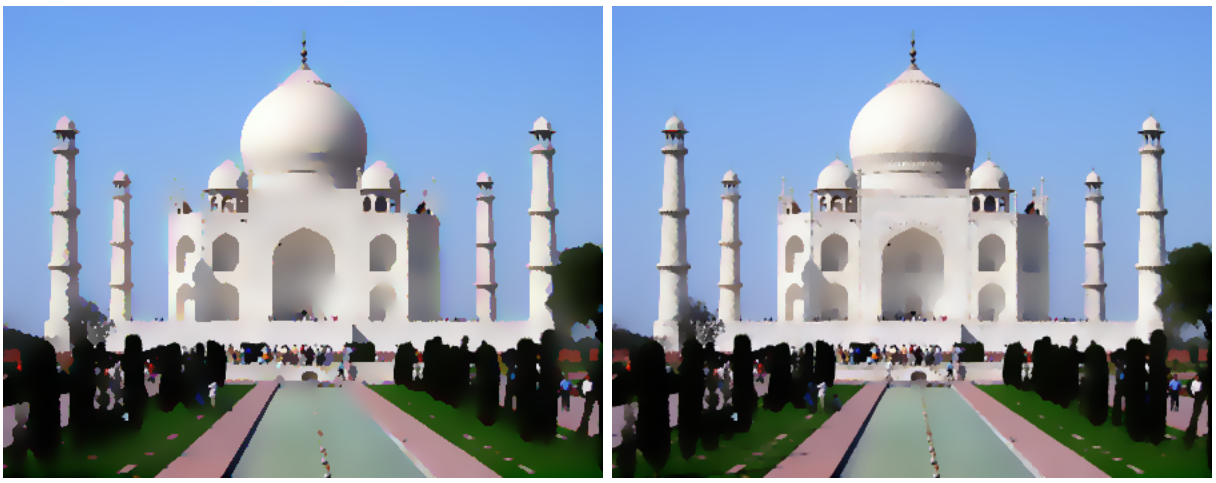
\includegraphics[scale=0.22]{effectofg.png} \caption{Images generated using the two proposed functions $g$ and $k=0.05$, at $t=128$. (Second is exponential.)}
    \end{figure}
    
        \begin{itemize}
            \item $e^{-\left(\frac{||\nabla I ||}{K}\right)^2}$ ``privileges high contrast edges over low contrast ones''
            \item $\frac{1}{1+\left(\frac{||\nabla I ||}{K}\right)^2}$ ``privileges wide regions over smaller ones''
        \end{itemize}

\end{frame}

%%%%%%%%%%%%%%%%%%%%%%%%%%%%%%%%
\begin{frame}{Experiments: The effect of the constant $K$}

        \begin{itemize}
            \item $K$ controls the width of $g$
            \item if an image is very noisy, need $g$ wide $\to K$ large; if it has little noise, need $g$ narrow $\to K$ small.
        \end{itemize}
    We can choose $K$ experimentally or using Canny noise estimation

\end{frame}

%%%%%%%%%%%%%%%%%%%%%%%%%%%%%%%%
\begin{frame}{Experiments: The effect of the constant $K$}

    \begin{figure}[h!]
            \centering            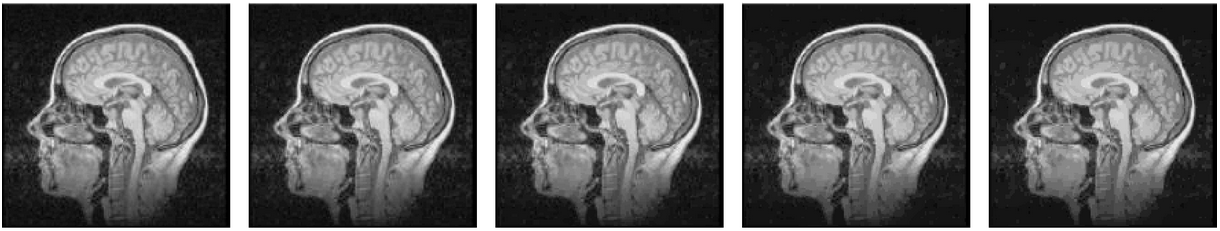
\includegraphics[scale=0.21]{effectofk1.png}
            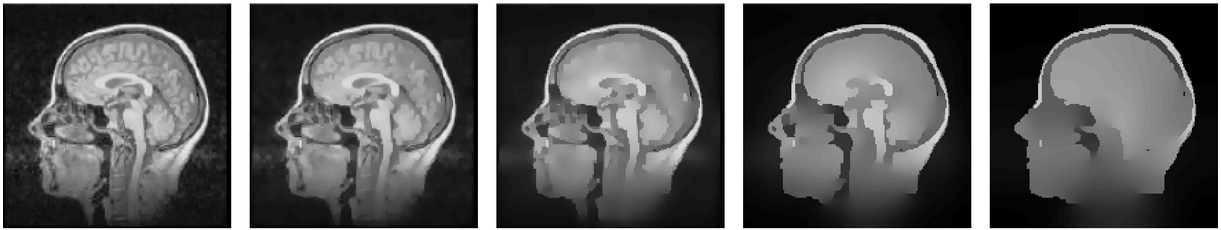
\includegraphics[scale=0.21]{effectofk2.png}
            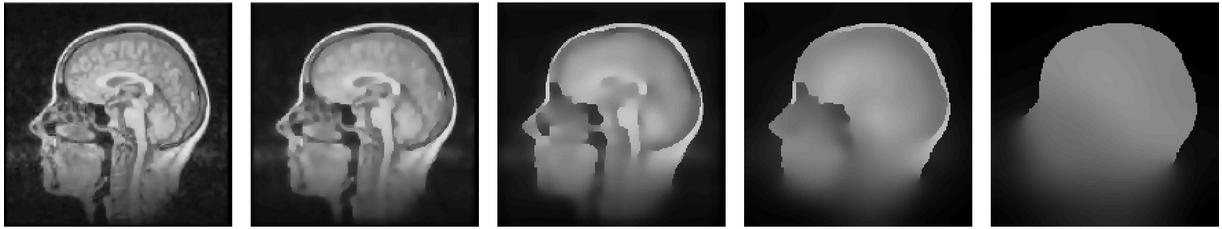
\includegraphics[scale=0.21]{effectofk3.png}
            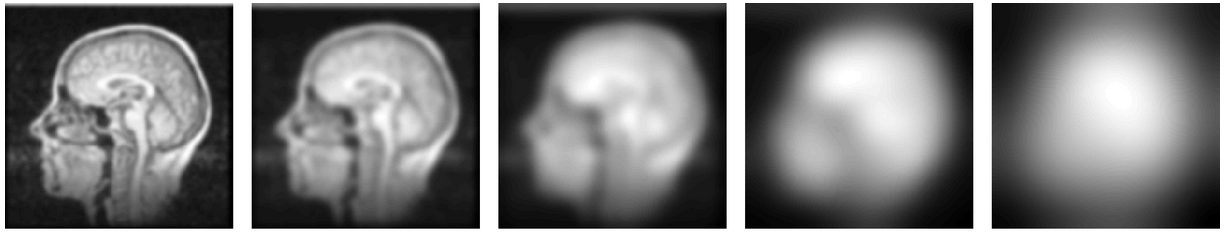
\includegraphics[scale=0.21]{effectofk4.png}
            \caption{Top row using $k=1$, then $k=7.66,14.32,100000$}
    \end{figure}

\end{frame}

%%%%%%%%%%%%%%%%%%%%%%%%%%%%%%%%
\begin{frame}{Properties}

    \begin{block}{Properties of the PDE problem}
        \begin{itemize}
            \item can prove that for either suggested $g$, the problem is well-posed and numerically stable if $K$ is chosen correctly
            \item other $g$ might also have good properties
        \end{itemize}
    \end{block}
    \begin{block}{Properties of the resulting family of images}
        \begin{itemize}
            \item can prove that edges are actually enhanced
            \item can prove that no new features are created
        \end{itemize}
    \end{block}

\end{frame}

%%%%%%%%%%%%%%%%%%%%%%%%%%%%%%%%
\begin{frame}{Applications}

        \begin{itemize}
            \item on its own, it makes images more clear
            \item in other algorithms, e.g., image segmentation, inpainting
            \item importantly, it can improve edge detection 
                \begin{itemize}
                    \item makes edges detected with gradients more meaningful
                \end{itemize}
        \end{itemize}
    \begin{figure}[h!]
        \centering            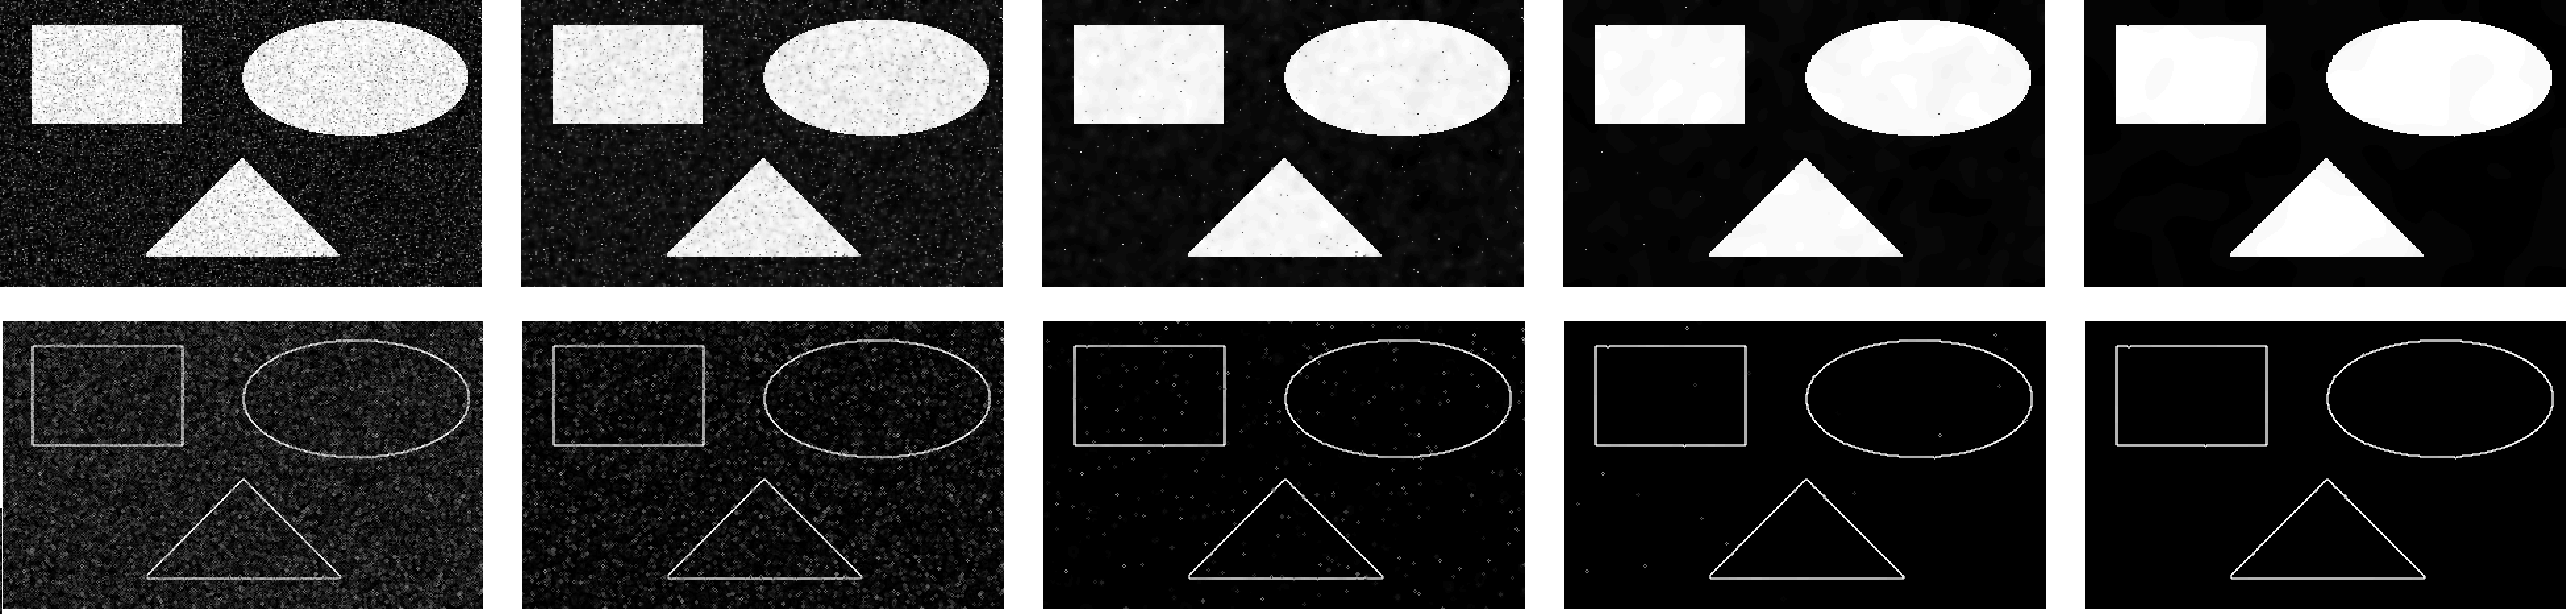
\includegraphics[width=10cm, height=4cm]{edgedetwdif.png}
        \caption{Top row: anisotropic diffusion; bottom row: edges recovered with gradient method}
    \end{figure}
    
\end{frame}

%%%%%%%%%%%%%%%%%%%%%%%%%%%%%%%%
\begin{frame}{Example implementation}

    \begin{block}{OpenCV's anisotropicDiffusion()}
        Parameters: 
        \begin{itemize}
            \item \textbf{src}\,\,\, Source image with 3 channels. 
            \item \textbf{dst}\,\,\, Destination image of the same size and the same number of channels as src . 
            \item \textbf{alpha}\,\,\, The amount of time to step forward by on each iteration (normally, it's between 0 and 1). 
            \item \textbf{K}\,\,\, sensitivity to the edges 
            \item \textbf{ninters}\,\,\, The number of iterations 
        \end{itemize}
    \end{block}

\end{frame}

%%%%%%%%%%%%%%%%%%%%%%%%%%%%%%%%
\begin{frame}{References}

    \begin{enumerate}
        \item Bertalmio, M. \& Bertozzi, Andrea \& Sapiro, G.. (2001). Navier-Stokes, fluid dynamics, and image and video inpainting. Proc. IEEE Comput. Soc. Conf. Comput. Vis. Pattern Recognit. 1. I-355. 10.1109/CVPR.2001.990497.
        \item Bin Zhou, Xiao-Lin Yang, Rui Liu and Wei Wei, 2010. Image Segmentation with Partial Differential Equations. Information Technology Journal, 9: 1049-1052.
        \item Pietro Perona and Jitendra Malik (July 1990). "Scale-space and edge detection using anisotropic diffusion". IEEE Transactions on Pattern Analysis and Machine Intelligence. 12 (7): 629–639.
        \item J Weickert, 2001. Efficient image segmentation using partial differential equations and morphology. Pattern Recognition Volume 34, Issue 9, September 2001, Pages 1813-1824
        \item Weickert, J.: Anisotropic diffusion in image processing. B.G. Teubner, Stuttgart (1998). 
    \end{enumerate}
\end{frame}

\begin{frame}{References}
    \begin{block}{Images only from}
    \begin{enumerate}
        \item Figures 1-3: https://github.com/polyfloyd/edge-detection-rs
        \item Figure 6: https://mipav.cit.nih.gov/pubwiki/index.php/ Filters\_(Spatial)\_Anisotropic\_Diffusion
        \item Figure 7: http://www.codebind.com/python/opencv-python-tutorial-beginners-smoothing-images-blurring-images-opencv/
        \item Figure 8: http://www.cs.utah.edu/~manasi/coursework/cs7960/p2/project2.html
        \item Figures 9-10: https://www.cs.utah.edu/~jfishbau/advimproc/project2/
    \end{enumerate}
    \end{block}

\end{frame}



\end{document}
